\subsubsection{Q10.20 data 11092021 grouped by scenario \& PGM}

\begin{comment}
                             EFPR        EO      EFNR     n    pvalue
(frauth, Advantaged)     0.538462  0.461538  0.461538  13.0  0.694887
(frauth, Disadvantaged)  0.388889  0.611111  0.500000   9.0  0.580712
(icu, Advantaged)        0.555556  0.444444  0.555556   9.0  0.359375
(icu, Disadvantaged)     0.437500  0.562500  0.750000   8.0  0.825432
(rent, Advantaged)       0.312500  0.687500  0.500000   8.0  0.162441
(rent, Disadvantaged)    0.500000  0.500000  0.400000  10.0  1.000000
\end{comment}

\begin{table}[h]
    \centering
    \begin{tabular}{|c|c|c|c|c|c|c|}
        \hline
        scenario & PGM & EFPR & EO & EFNR & n & p-value\\
        \hline
        frauth & Advantaged & \textbf{0.538} & 0.462 & 0.462 & 13.0 & 0.695\\
		frauth & Disadvantaged & 0.389 & \textbf{0.611} & 0.500 & 9.0 & 0.581\\
		icu & Advantaged & \textbf{0.556} & 0.444 & \textbf{0.556} & 9.0 & 0.359\\
		icu & Disadvantaged & 0.438 & \textbf{0.562} & \textbf{0.750} & 8.0 & 0.825\\
		rent & Advantaged & 0.312 & \textbf{0.688} & 0.500 & 8.0 & 0.162\\
		rent & Disadvantaged & 0.500 & 0.500 & 0.400 & 10.0 & 1.000\\
		
        \hline
    \end{tabular}
    \caption{Grouped by scenario PGM}
    \label{tab:my_label}
\end{table}
\begin{figure}[h]
    \centering
    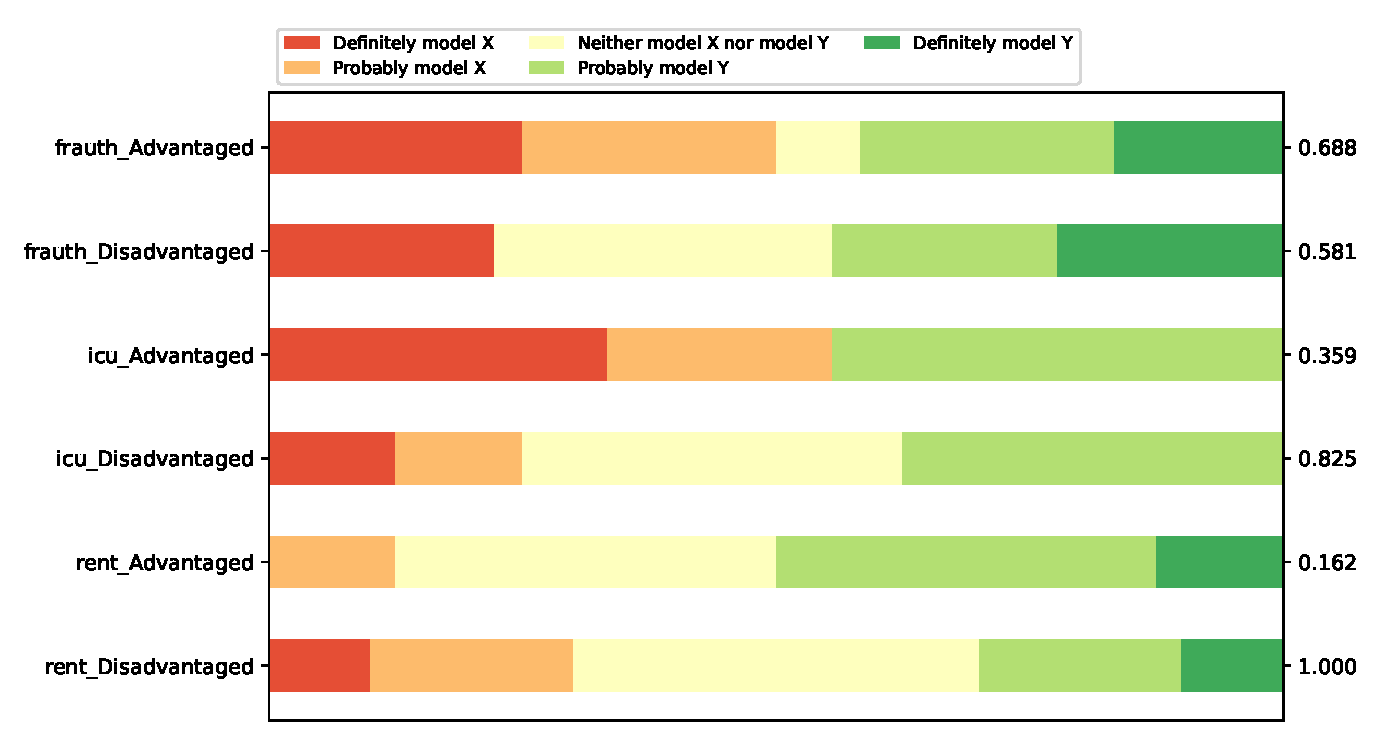
\includegraphics[width=0.8\textwidth]{figures/Q10.20/11092021/Q10.20_scenario_PGM.pdf}
    \caption{Grouped by scenario \& PGM}
    \label{fig:my_label}
\end{figure}
